%-----------------------------------------------------------------------
% 
%-----------------------------------------------------------------------
%
%     
%
%
%%%%%%%%%%%%%%%%%%%%%%%%%%%%%%%%%%%%%%%%%%%%%%%%%%%%%%%%%%%%%%%%%%%%%%%%


\documentclass[twoside]{article}
\usepackage{amsmath,amsthm,amssymb,verbatim}

%     If your article includes graphics, uncomment this command.
\usepackage{graphicx}

%     If the article includes commutative diagrams, ...
%\usepackage[cmtip,all]{xy}

\usepackage{url}

\usepackage{fancyhdr}
\pagestyle{fancy}

\def\blfootnote{\xdef\@thefnmark{}\@footnotetext} 
\long\def\symbolfootnote[#1]#2{\begingroup%
\def\thefootnote{\fnsymbol{footnote}}\footnote[#1]{#2}\endgroup} 

	\addtolength{\oddsidemargin}{1cm}
	\addtolength{\evensidemargin}{-1cm}

\setcounter{page}{1}

\begin{document}

%     If you need symbols beyond the basic set, uncomment this command.
%\usepackage{amssymb}


\newtheorem{theorem}{Theorem}[section]
\newtheorem{lemma}[theorem]{Lemma}

\theoremstyle{definition}
\newtheorem{definition}[theorem]{Definition}
\newtheorem{example}[theorem]{Example}
\newtheorem{xca}[theorem]{Exercise}

\theoremstyle{remark}
\newtheorem{remark}[theorem]{Remark}

\numberwithin{equation}{section}


\date{}
\lhead[]{}
\chead[\underline{Universality }]{\it{O. Shanker}}
\rhead[]{}

% \title[short text for running head]{full title}
\title{\bf{Universality of Riemann Zeta Function value distribution on critical axis}}

\maketitle


%    author one information
% \author[short version for running head]{name for top of paper}
\author{{\textbf{O. Shanker}},}
\thanks{ Mountain View, CA 94041, U. S. A. email: oshanker@gmail.com}

\thispagestyle{fancy}

%    Abstract is required.
\begin{abstract}
We present a remarkable and striking universality property for the value distribution
of the Riemann zeta function on the critical axis.

\end{abstract}
{\textbf {Keywords}:} Riemann zeta, Value Distribution, Universality, Hardy's function
{\textbf {Mathematics Subject Classification (MSC)}:} 11M06, 11-04.


\symbolfootnote[0]{\bf{* }}


\section{Introduction}

The universality relations and symmetries exhibited by a system are fundamental aspects of the system. 
In this work, we present a universality relation for the value
distribution of the Hardy $Z$ function at Generalized Gram points.

Ref.~\cite{Shanker 2018a} studied empirically the distribution of $Z(t)$ values at Gram points and
showed  that the distribution for even Gram points was the negative  of the distribution for odd Gram points. 
Ref.~\cite{Shanker 2018b}) extended the study to Generalized Gram points and showed 
that the  value
distribution of the Hardy $Z$ function at discrete points is anti-symmetrical for reflections around the mid-points 
of 
the Gram intervals (Eq.~\ref{eq:antisym}) and symmetrical for reflections around the Gram points(Eq.~\ref{eq:sym}). 

\begin{figure*}
\centering
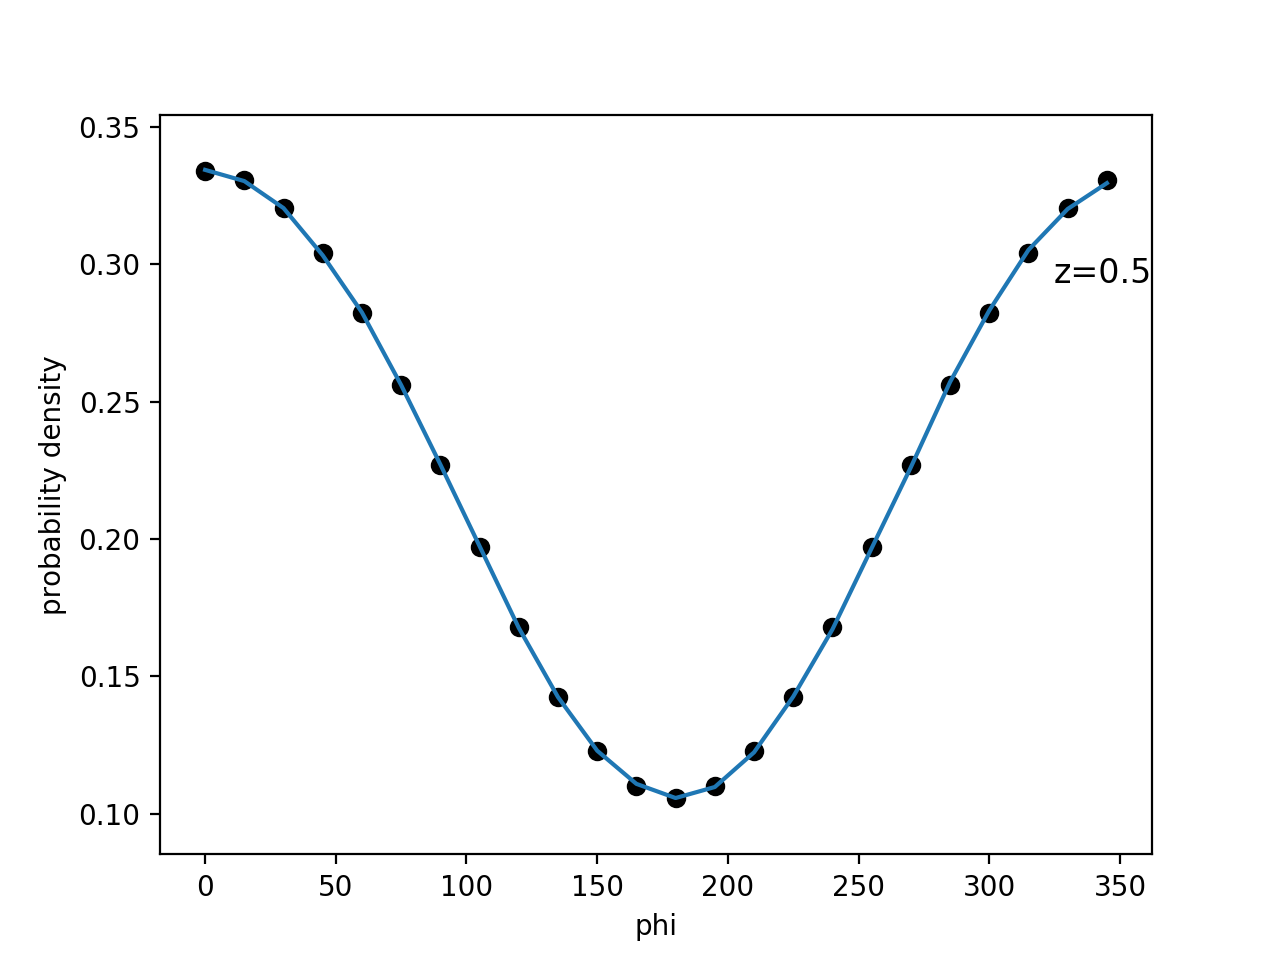
\includegraphics[width=0.8\textwidth]{z05.png}
\caption[]{ 
 Test of universality. Comparison of probability density prediction from
 universality with actual values, for $z=0.5$. The y axis is the probability density.
 The x axis is the angle characterizing the Generalized Gram point.
  }
\vspace{1mm}
\label{z05}
\end{figure*}

\begin{figure*}
\centering
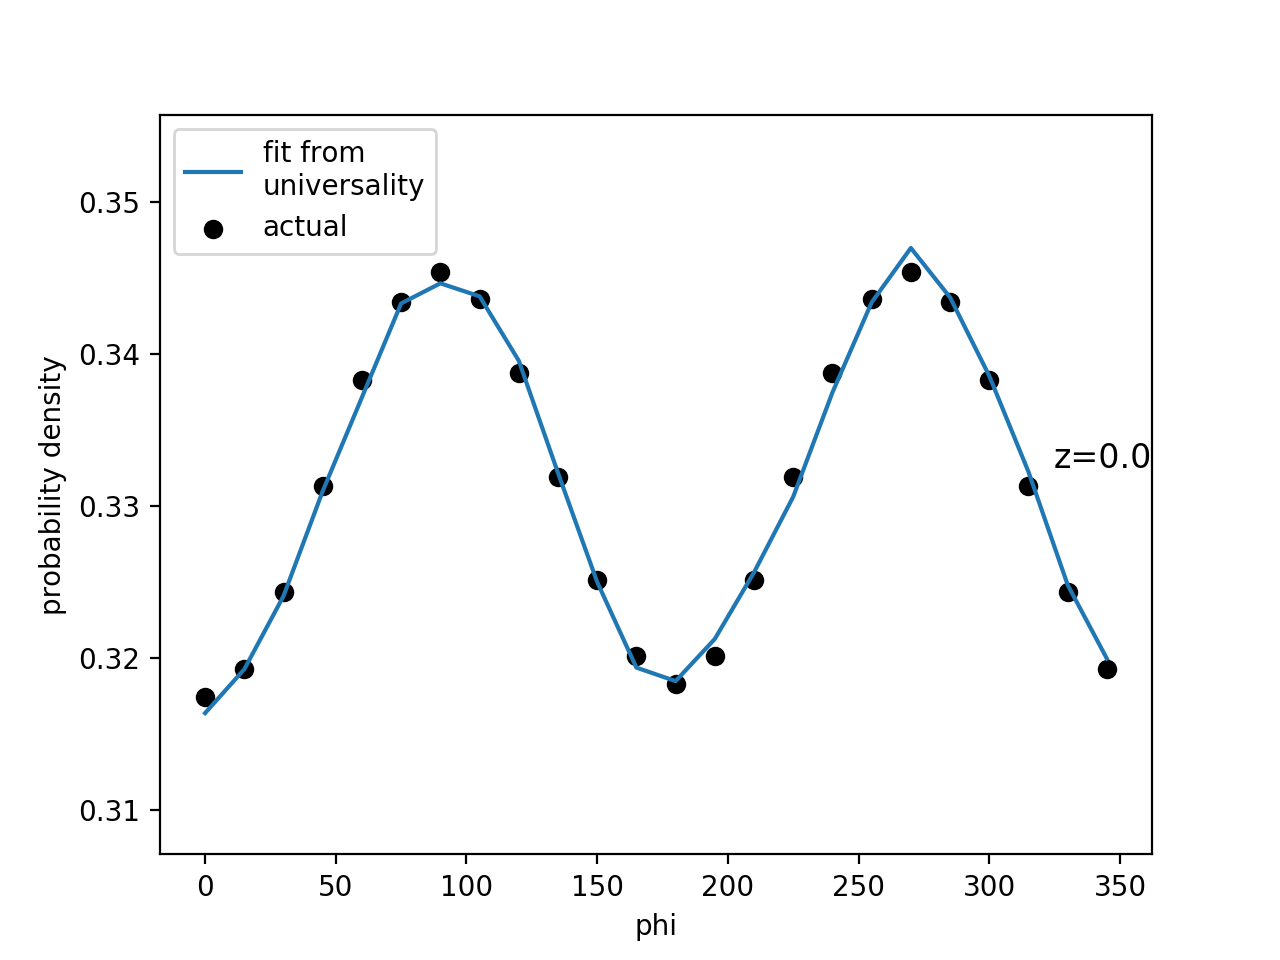
\includegraphics[width=0.8\textwidth]{z00.png}
\caption[]{ 
 Test of universality. Comparison of probability density prediction from
 universality with actual values, for $z=0.0$. 
  }
\vspace{1mm}
\label{z00}
\end{figure*}

\section{\label{sec2}Notation for the Riemann zeta function}

In this section we  establish the required notation for the 
Riemann Zeta Function. 
For $\mathrm{Re} (s) > 1$ the Riemann Zeta function is defined as
\begin{equation}
\zeta ( s ) \, = \, \sum^{\infty}_{n = 1} \; n^{-s} \, = \, \prod_{p \in primes} \;
\left( 1 - p^{-s} \right)^{-1}.
\label{eqRie}
\end{equation}
 $\zeta ( s )$ can be continued to
the complex plane. Riemann's hypothesis, that the non-trivial zeros of $\zeta ( s )$ lie on the 
critical axis $1/2+it$, is probably the most famous unsolved problem in mathematics.
The mean spacing $\delta$ of the zeros  at large height $T$ is $\delta = 2\pi(\ln (T/2\pi))^{-1}$. 
For numerical studies of the Riemann hypothesis one defines Hardy's function
\begin{equation}
Z(t)=exp(i\theta(t))\zeta(1/2 +it) 
\label{eq:hardy}
\end{equation}
where 
\begin{equation}
\theta(t) = arg (\pi^{it/2} \Gamma(\frac{1}{4} + \frac{it}{2})). 
\label{eq:theta}
\end{equation}
The argument in Eq.~\ref{eq:theta} is defined by continuous variation of $t$ starting with the value $0$ at $t = 0$.
$Z(t)$ is real valued for real $t$,
and we have $|Z(t)| = |\zeta(1/2+it)|$. Thus the zeros of $Z(t)$ are the imaginary part of the zeros 
of $\zeta(s)$ which lie on the critical line.  

Gram points~\cite{Gram 1903} play an important role in the the theory because many of the zeros are separated by them.  When $t \ge 7$, the $\theta$ function Eq.(\ref{eq:theta}) is monotonic increasing. 
For $n \ge -1$, the $n$-th Gram point $g_n$ is defined as the unique solution $> 7$ to
$\theta (g_n) = n\pi$. A Gram interval is the interval $G_n = [g_n,g_{n+1})$.
 In analogy with Gram points, we can associate an angle $\phi$ with a point $t$ on the critical axis as follows:
\begin{definition}\label{phi}
For $t \ge 7$, $t$ is said to be a generalized Gram point with value $\phi$  if
$\theta (t) = 2k\pi + \phi$, where $0 \le \phi < 2\pi$.
\end{definition}


\section{\label{sec3}Probability Distribution}
In this section 

The sample space for our study is the interval along the critical axis specified by $(T_1, T_2)$. 
While empirical studies necessarily use large but finite  $T_1, T_2$, we are interested in the limit 
$T_1 \rightarrow \infty, T_2 \rightarrow \infty,  T_2-T_1 \rightarrow \infty,$ however
\begin{equation}
T_2 - T_1  \ll T_1. 
\label{eq:interval}
\end{equation}
Because of Equation \ref{eq:interval}, we can consider  $\ln (t)$  to be effectively constant over  the interval.
The latter condition is not essential but is convenient, in that it simplifies the numerical work. 
The notation $\ln (t)$ stands for the natural logarithm of $t$.  
We study the probability distribution function for $Z(t)$ at generalized Gram  points,
 $p_{\phi}(y)$:
\begin{definition}\label{pphi}
\begin{equation}
\int\limits_{a}^{b} p_{\phi}(z)dz
\label{eq:pdfphi}
\end{equation}
is the probability that $a<Z(t)<b$ when we consider the values of $Z(t)$ for a large number of 
generalized Gram points in the sample space. 
\end{definition}
The probability density  $p_{\phi}(z)$ depends on the sample space (i.e., on the height $t$ and on the size of 
the sample space). In practice the densities are not sensitive to the choice of the sample space as long as 
the height $t$ is large enough and the length of the interval from which the sample is collected is large enough 
(but not too large on log scale). The emphasis in this work is on the empirical study of the distribution. 
There are important open theoretical questions about the distribution that we do not cover, 
and we mention those questions in the Appendix.


The anti-symmetry relation is
\begin{equation}
p_{\phi}(z) = p_{\phi+\pi}(-z).
\label{eq:antisym}
\end{equation}
The symmetry relation ius
\begin{equation}
p_{\phi}(z) = p_{2\pi-\phi}(z).
\label{eq:sym}
\end{equation}



We briefly mention other studies of the value distribution of the Riemann zeta function and the closely related Hardy's function~\cite{Hardy 1918}.  Ivi\'c's monograph~\cite{Ivic 2013} has a comprehensive survey of  the field.
Selberg in unpublished work showed that at large $t$ $\log (\zeta(\frac{1}{2} + it))$ is approximately normally distributed with a standard deviation of order $\sqrt{log~log~t}$ (see Ref.~\cite{Hejhal}). He showed a 
similar result~\cite{Selberg 1989, Selberg 1991} for $\log (|Z(t)|)$. Laurincikas~\cite{Laurincikas}  used probabilistic number theory to prove various results about the distribution of the Riemann zeta function.

Regarding the value distribution at specific points along the Gram interval, 
Titchmarsh~\cite{Titchmarsh 1934} and Kalpokas and Steuding~\cite{kalpokas 2009} present 
results pertaining to the
mean value of the Riemann zeta function. Lester's~\cite{Lester 2013} Ph. D. thesis also 
considers the distribution of $\log (|\zeta(\frac{1}{2} + it)|)$  for specific points along the Gram interval.  
The question of the values of Hardy's $Z$-function at a discrete sequence of points on the critical axis 
is quite interesting. The above references give some results in this direction that can be proved rigorously. 
At the same time, the present state of Riemann zeta function theory gives limited information 
about the value distribution of $Z(t)$ at discrete sequences of points. Possibly, these analogues 
could differ significantly from the continuous case.  
Our numerical studies of the value distribution of Hardy's $Z$-function at discrete points
helps fill the gaps. 



\begin{table}
\centering \(\begin{array}{ccccccc}
\hline
 \phi &     Min.   &  \multicolumn{2}{c}  {Median }   &   Mean   &  \multicolumn{2}{c}  {Max.} \\
  \cline{3-7}  
 &              & Quantile   &      x      &              & Quantile.    &  y \\
\hline
0 &-69 &0.1134 &0.8517 &2.0001 &2.5403 &165  \\
\pi/4 &-97 &-0.1352 &0.5916 &1.4143 &2.1226 &159 \\
\hline
\end{array}\)
\caption{Quantiles and mean for  $Z(t)$ when $\phi$ values are multiples of $\pi/4$.} 
\label{tab:multicolumn}
\end{table}



Hardy's function $Z(t)$  is evaluated using the Riemann$-$Siegel series
\begin{equation}
Z(t) = 2\sum^{m}_{n=1}\frac{\cos(\theta(t) - t \ln (n))}{\sqrt{n}} + R(t), 
\label{eq:RS}
\end{equation}
where $m$ is the integer part of $\sqrt{t/(2\pi)}$. $R(t)$ is a small remainder
term which can be evaluated to the desired level of accuracy. We used the techniques in
 Refs.~\cite{Odlyzko 1992,hiary,gourdon} 
to efficiently evaluate the zeta function at large $t$. To evaluate  $Z(t)$  at several points 
in the Gram interval, we have to use band limited function interpolation~\cite{Jerri 1977}. 
We evaluate the coefficients in the series for band limited function interpolation at the Gram points, 
and use the series to evaluate $Z(t)$ at other points in the Gram interval. The most important 
source for loss of accuracy at large heights is the cancellation between
large numbers that occur in the arguments of the $\cos$ terms in Eq.~(\ref{eq:RS}). We 
use a high precision module to evaluate the arguments. The rest of the calculation
is done using regular double precision accuracy. The  zeros from Ref~\cite{hiary 2010} were used 
to check the accuracy of our zeta function calculations. Our evaluations of $Z(t)$ at $T=10^{12}$ 
are accurate 
to better than $10^{-6}$. 



\begin{table}
\centering \(\begin{array}{cccccccccccc}

\hline
0&\pi/6 &\pi/3 &\pi/2 &2\pi/3 &5\pi/6 &\pi &7\pi/6 &4\pi/3 &3\pi/2 &5\pi/3 &11\pi/6 \\
\hline
1.995&1.728&0.997&-0.002&-1.000&-1.731&-1.999&-1.731&-1.000&-0.002&0.997&1.728 \\
7.886&7.816&7.882&8.011&8.054&7.980&7.858&7.796&7.877&8.022&8.078&8.010 \\
\hline
\end{array}\)
\caption{Mean    $Z(t)$ and Standard Deviation at $T=10^{28}$. Row 1: $\phi$, Row 2: mean~$Z$, Row 3: Standard Deviation}
\label{tab:mean28}
\end{table}



\section{\label{conclusions}Conclusions}

The most exciting new result is the discovery of a universality relation for the 
value distribution of the Hardy Z function at discrete points. 

\section*{\label{appendix} Appendix}

A more precise definition for the function $p_{\phi}(y)$ is provided. We consider the interval along 
the critical axis specified by $(T_1, T_2)$. While empirical studies necessarily use large but 
finite  $T_1, T_2$, we are interested in the limit 
$T_1 \rightarrow \infty, T_2 \rightarrow \infty,  T_2-T_1 \rightarrow \infty,$ however
\begin{equation}
T_2 - T_1  \ll T_1. 
\label{eq:interval}
\end{equation}
Because of Equation \ref{eq:interval}, we can consider  $\ln (t)$  to be effectively constant over  the interval. A probability space $W$ is defined by a sample space of elementary events $\Omega$, a $\sigma$ algebra of all considered events $\mathcal{F}$, and a probability measure $P$. Our space of elementary events $\Omega$ is the set of all generalized Gram points with value phi in the interval. This is easily seen to be a discrete space. If we denote $\theta (T_1) = 2k_1\pi + \phi$, $\theta (T_2) = 2k_2\pi + \phi$, then we can index the set of generalized Gram points in the interval by the integer  $k$, where $k$ lies in the interval $(k_1, k_2)$. Since the mean spacing $\delta$ of the zeros at height $t$ is $\delta = 2\pi(\ln (t/2\pi))^{-1}$, the cardinality of this set is $(T_2 - T_1)*(\ln (T_1/2\pi))/(2\pi)$. Since we are dealing with a discrete space, we follow standard practice and choose $\mathcal{F}$,  the  $\sigma$ algebra, to be the collection of all subsets of $\Omega$ . Finally, the random variable whose probability distribution we wish to study is the value of $Z(t)$ at the generalized Gram point $t$.


We can get some insight into the probability distribution $p_{\phi}(z)$ from the studies of 
Kalpokas and Steuding \cite{kalpokas 2009}. 
They show that for $\phi_1$ in the range $[0, \pi)$ 
\begin{equation}
\sum_{0 < t < T, \zeta(\frac{1}{2}+it) \in e^{i\phi_1}\mathbb{R}} \zeta(\frac{1}{2}+it) = (2e^{i\phi_1}\cos(\phi_1))\frac{T}{2\pi}\ln (\frac{T}{2\pi}) + O_\epsilon(T^{(\frac{1}{2}+\epsilon}).
\label{eq:kalpokas1}
\end{equation}
From Equation~\ref{eq:kalpokas1} and the cardinality of our sample space, it follows that a finite mean can be defined for the value distribution in our sample space. This gives support to the existence of a limiting distribution. We now consider the possibility of defining higher order moments for the value distribution. Kalpokas and Steuding  also show that
\begin{equation}
\sum_{0 < t < T, \zeta(\frac{1}{2}+it) \in e^{i\phi_1}\mathbb{R}} |\zeta(\frac{1}{2}+it)|^2 = \frac{T}{2\pi}(\ln (\frac{T}{2\pi}))^2 + (2\gamma+2\cos(2\phi_1))\frac{T}{2\pi}\ln (\frac{T}{2\pi}) + \frac{T}{2\pi} + O_\epsilon(T^{(\frac{1}{2}+\epsilon}),
\label{eq:kalpokas2}
\end{equation}
where $\gamma$ is Euler's constant. From Equation~\ref{eq:kalpokas2} and the cardinality of our sample space 
it seems that higher order moments of the value distribution diverge logarithmically. 
There is a lot of cancellation between positive and negative values of $Z(T)$ for odd moments, 
so odd moments will  behave better than even moments. It seems likely that a limiting value distribution exists, 
it has a finite well-defined mean, and higher moments diverge logarithmically. 
Distributions which do not have all moments defined are used in applications, for example, 
the Cauchy-Lorentz distribution~\cite{feller}. Equation~\ref{eq:kalpokas1} and \ref{eq:kalpokas2} 
predict that the standard deviation should be independent of $\phi$. 
These equations also imply that the probability distribution will have a finite standard deviation if the 
argument is normalized by $\sqrt{\frac{T}{2\pi}}$.
 


\bibliographystyle{amsplain}
\begin{thebibliography}{10}

\bibitem{Gram 1903} J. P. Gram, 
``Sur les Zeros de la Fonction  $\zeta ( s )$  de Riemann",
{\it Acta Math.} {\bf27}(1903), 289-304

\bibitem{Titchmarsh 1934} E. C. Titchmarsh,
``On van der Corput's method and the zeta-function of Riemann (IV)",
{\it Quart. J. Math. Oxford Ser.} {\bf5}(1934), 98-105

\bibitem{Shanker 2018a} O. Shanker, 
``Good to Bad Gram Point Ratio For Riemann Zeta Function",
{\it Experimental Mathematics} {\bf doi:10.1080/10586458.2018.1492474}(2018)

\bibitem{Shanker 2018b} O. Shanker, ``Symmetry properties of distribution of Riemann Zeta Function values on critical axis''
{\it Advanced Modeling and Optimization}, {\bf 20}, 435-445, (2018). 


\bibitem{hiary 2010} G. A. Hiary,
``An amortized-complexity method to compute the Riemann zeta function", 
{\it Mathematics of Computation} {\bf80}(2011), 1785-1796


\bibitem{Hardy 1918} G. H. Hardy and J. E. Littlewood,
``Contributions to the theory of the Riemann
zeta-function and the distribution of primes",
{\it Acta Math.} {\bf41}(1918), 119-196

\bibitem {Ivic 2013} Aleksandar Ivi\'c, ``The Theory of Hardy's Z-Function,''
Cambridge University Press,  (2013)

\bibitem{Hejhal} D. A. Hejhal,
``On a result of Selberg concerning zeros of linear combinations
of L-functions", 
{\it Int. Math. Res. Not.} {\bf11}(2000), 551-577

\bibitem {Selberg 1989} A. Selberg, ``Selected Papers, Vol. I,''
Springer Verlag,  (1989)

\bibitem {Selberg 1991} A. Selberg, ``Selected Papers, Vol. II,''
Springer Verlag,  (1991)



\bibitem{Laurincikas} A. Laurincikas,
``Limit Theorems for the Riemann Zeta-Function",
Kluwer, Dordrecht, 1996

\bibitem{kalpokas 2009} J. Kalpokas and J. Steuding,
``On the value-distribution of the Riemann zeta-function on the critical line", 
{\it Moscow Journal of Combinatorics and
Number Theory} {\bf1}(2011), 26-42

\bibitem {Lester 2013} Stephen J. Lester, ``The Distribution of Values of the
Riemann Zeta-Function,''
Ph. D. dissertation, University of Rochester,  (2013)

\bibitem{Odlyzko 1992}  A. Odlyzko,
``The $10^{20}$-th Zero of the Riemann Zeta
Function and 175 Million of its Neighbors", report,
\url{http://www.dtc.umn.edu/~odlyzko/unpublished/zeta.10to20.1992.pdf}, (1992)

\bibitem{hiary} G. A. Hiary,
``Fast methods to compute the Riemann zeta function",
{\it Annals of Mathematics} {\bf74}(2011), 891-946

\bibitem{gourdon} Xavier Gourdon,
``The $10^{13}$ first zeros of the Riemann Zeta function,
and zeros computation at very large height", report,
\url{http://numbers.computation.free.fr/Constants/Miscellaneous/zetazeros1e13-1e24.pdf}, (2004)

\bibitem{Jerri 1977} A. J. Jerri,
``The Shannon sampling theorem - its various extensions and applications",
{\it Proc IEEE} {\bf65}(1977), 1565-1596

\bibitem{feller} William Feller,
``An Introduction to Probability Theory and Its Applications, Volume II (2 ed.)",
John Wiley and Sons, New York, 1971


\end{thebibliography} 

\end{document}
